%File: anonymous-submission-latex-2025.tex
\documentclass[letterpaper]{article} % DO NOT CHANGE THIS
\usepackage[submission]{aaai25}  % DO NOT CHANGE THIS
\usepackage{times}  % DO NOT CHANGE THIS
\usepackage{helvet}  % DO NOT CHANGE THIS
\usepackage{courier}  % DO NOT CHANGE THIS
\usepackage[hyphens]{url}  % DO NOT CHANGE THIS
\usepackage{graphicx} % DO NOT CHANGE THIS
\urlstyle{rm} % DO NOT CHANGE THIS
\def\UrlFont{\rm}  % DO NOT CHANGE THIS
\usepackage{natbib}  % DO NOT CHANGE THIS AND DO NOT ADD ANY OPTIONS TO IT
\usepackage{caption} % DO NOT CHANGE THIS AND DO NOT ADD ANY OPTIONS TO IT
\frenchspacing  % DO NOT CHANGE THIS
\setlength{\pdfpagewidth}{8.5in} % DO NOT CHANGE THIS
\setlength{\pdfpageheight}{11in} % DO NOT CHANGE THIS
%
% These are recommended to typeset algorithms but not required. See the subsubsection on algorithms. Remove them if you don't have algorithms in your paper.
\usepackage{algorithm}
\usepackage{algorithmic}

%
% These are are recommended to typeset listings but not required. See the subsubsection on listing. Remove this block if you don't have listings in your paper.
\usepackage{newfloat}
\usepackage{listings}
\DeclareCaptionStyle{ruled}{labelfont=normalfont,labelsep=colon,strut=off} % DO NOT CHANGE THIS
\lstset{%
	basicstyle={\footnotesize\ttfamily},% footnotesize acceptable for monospace
	numbers=left,numberstyle=\footnotesize,xleftmargin=2em,% show line numbers, remove this entire line if you don't want the numbers.
	aboveskip=0pt,belowskip=0pt,%
	showstringspaces=false,tabsize=2,breaklines=true}
\floatstyle{ruled}
\newfloat{listing}{tb}{lst}{}
\floatname{listing}{Listing}
%
% Keep the \pdfinfo as shown here. There's no need
% for you to add the /Title and /Author tags.
\pdfinfo{
/TemplateVersion (2025.1)
}
\usepackage{makecell}
% \usepackage{cleveref}
\usepackage{xcolor}         % colors

\definecolor{c1}{HTML}{801dae}
\definecolor{c2}{HTML}{008000}
\definecolor{c3}{HTML}{00BFFF}
\definecolor{c4}{HTML}{0c8918}

\newcommand{\secref}[1]{Sec. \ref{#1}}
\newcommand{\figref}[1]{Figure \ref{#1}}
\newcommand{\eqnref}[1]{Eq. (\ref{#1})}
\newcommand{\tabref}[1]{Table \ref{#1}}
\newcommand{\exref}[1]{Example \ref{#1}}
\newcommand{\MY}[1]{\textcolor{teal}{[MY: #1]}}
\newcommand{\KZ}[1]{\textcolor{blue}{[Kenny: #1]}}
\newcommand{\XJ}[1]{\textcolor{orange}{[Xiujie: #1]}}


% \usepackage[T1]{fontenc}


% DISALLOWED PACKAGES
% \usepackage{authblk} -- This package is specifically forbidden
% \usepackage{balance} -- This package is specifically forbidden
% \usepackage{color (if used in text)
% \usepackage{CJK} -- This package is specifically forbidden
% \usepackage{float} -- This package is specifically forbidden
% \usepackage{flushend} -- This package is specifically forbidden
% \usepackage{fontenc} -- This package is specifically forbidden
% \usepackage{fullpage} -- This package is specifically forbidden
% \usepackage{geometry} -- This package is specifically forbidden
% \usepackage{grffile} -- This package is specifically forbidden
% \usepackage{hyperref} -- This package is specifically forbidden
% \usepackage{navigator} -- This package is specifically forbidden
% (or any other package that embeds links such as navigator or hyperref)
% \indentfirst} -- This package is specifically forbidden
% \layout} -- This package is specifically forbidden
% \multicol} -- This package is specifically forbidden
% \nameref} -- This package is specifically forbidden
% \usepackage{savetrees} -- This package is specifically forbidden
% \usepackage{setspace} -- This package is specifically forbidden
% \usepackage{stfloats} -- This package is specifically forbidden
% \usepackage{tabu} -- This package is specifically forbidden
% \usepackage{titlesec} -- This package is specifically forbidden
% \usepackage{tocbibind} -- This package is specifically forbidden
% \usepackage{ulem} -- This package is specifically forbidden
% \usepackage{wrapfig} -- This package is specifically forbidden
% DISALLOWED COMMANDS
% \nocopyright -- Your paper will not be published if you use this command
% \addtolength -- This command may not be used
% \balance -- This command may not be used
% \baselinestretch -- Your paper will not be published if you use this command
% \clearpage -- No page breaks of any kind may be used for the final version of your paper
% \columnsep -- This command may not be used
% \newpage -- No page breaks of any kind may be used for the final version of your paper
% \pagebreak -- No page breaks of any kind may be used for the final version of your paperr
% \pagestyle -- This command may not be used
% \tiny -- This is not an acceptable font size.
% \vspace{- -- No negative value may be used in proximity of a caption, figure, table, section, subsection, subsubsection, or reference
% \vskip{- -- No negative value may be used to alter spacing above or below a caption, figure, table, section, subsection, subsubsection, or reference

\setcounter{secnumdepth}{2} %May be changed to 1 or 2 if section numbers are desired.

% The file aaai25.sty is the style file for AAAI Press
% proceedings, working notes, and technical reports.
%

% Title

% Your title must be in mixed case, not sentence case.
% That means all verbs (including short verbs like be, is, using,and go),
% nouns, adverbs, adjectives should be capitalized, including both words in hyphenated terms, while
% articles, conjunctions, and prepositions are lower case unless they
% directly follow a colon or long dash
% \title{AAAI Press Anonymous Submission\\Instructions for Authors Using \LaTeX{}}
\title{A Cognitive Evaluation Benchmark of Image Reasoning and Description for Large Vision-Language Models}

\author{
    %Authors
    % All authors must be in the same font size and format.
    Written by AAAI Press Staff\textsuperscript{\rm 1}\thanks{With help from the AAAI Publications Committee.}\\
    AAAI Style Contributions by Pater Patel Schneider,
    Sunil Issar,\\
    J. Scott Penberthy,
    George Ferguson,
    Hans Guesgen,
    Francisco Cruz\equalcontrib,
    Marc Pujol-Gonzalez\equalcontrib
}
\affiliations{
    %Afiliations
    \textsuperscript{\rm 1}Association for the Advancement of Artificial Intelligence\\
    % If you have multiple authors and multiple affiliations
    % use superscripts in text and roman font to identify them.
    % For example,

    % Sunil Issar\textsuperscript{\rm 2},
    % J. Scott Penberthy\textsuperscript{\rm 3},
    % George Ferguson\textsuperscript{\rm 4},
    % Hans Guesgen\textsuperscript{\rm 5}
    % Note that the comma should be placed after the superscript

    1101 Pennsylvania Ave, NW Suite 300\\
    Washington, DC 20004 USA\\
    % email address must be in roman text type, not monospace or sans serif
    proceedings-questions@aaai.org
%
% See more examples next
}

%Example, Single Author, ->> remove \iffalse,\fi and place them surrounding AAAI title to use it
\iffalse
\title{My Publication Title --- Single Author}
\author {
    Author Name
}
\affiliations{
    Affiliation\\
    Affiliation Line 2\\
    name@example.com
}
\fi

\iffalse
%Example, Multiple Authors, ->> remove \iffalse,\fi and place them surrounding AAAI title to use it
\title{My Publication Title --- Multiple Authors}
\author {
    % Authors
    First Author Name\textsuperscript{\rm 1},
    Second Author Name\textsuperscript{\rm 2},
    Third Author Name\textsuperscript{\rm 1}
}
\affiliations {
    % Affiliations
    \textsuperscript{\rm 1}Affiliation 1\\
    \textsuperscript{\rm 2}Affiliation 2\\
    firstAuthor@affiliation1.com, secondAuthor@affilation2.com, thirdAuthor@affiliation1.com
}
\fi


% REMOVE THIS: bibentry
% This is only needed to show inline citations in the guidelines document. You should not need it and can safely delete it.
\usepackage{bibentry}
% END REMOVE bibentry

\begin{document}

\maketitle

%\begin{abstract}
%  In the age of information explosion, search engines have been an
%  essential tool in people's daily life and query suggestion is one
%  of most useful feature for a standard search engine. However, because
%  most of search engines are keyword-based, many fantastic features would
%  fail when facing concept-based queries, so does query suggestion. In this
%  paper, we propose a framework so that search engines can give acceptable
%  suggestions when facing concept-based queries.
%\end{abstract}

\begin{abstract}
  A class of search queries which contain abstract concepts are studied in
this paper. These queries cannot be correctly interpreted by traditional keyword-based search engines.
  This paper presents a simple framework that detects and instantiates the
abstract concepts by their concrete entities or meanings to produce alternate
queries that yield better search results.
\footnote{Kenny Q. Zhu (corresponding author) is partially
supported by NSFC grants 61100050 and 61033002.}
\end{abstract}


\section{Introduction}

Protein$-$protein interactions (PPIs) are of central importance for the majority of biological functions, such as signal transduction, metabolic pathways, molecular dynamics, and protein networks\cite{Hoffmann.Krallinger.ea:2005}, for they serve as the most fundamental building blocks of the entire interacademic systems of any organisms. Collecting data on pairwise interaction relationships is essential for multiple purpose, including identification of modules with certain functionality\cite{Spirin.Mirny.03}, mapping diseases to dominated genes\cite{Ideker.Sharan.08}, and after all, understanding wholistic metabolic/genetic networks from a system biology perspective.

A lot of databases have been built to store protein and genetic interactions from major model organism species and are available in various standardized formats, such as MINT\cite{Zanzoni.Montecchi-Palazzi.ea:2002}, BIND\cite{Bader.ea:2003}, BIOGRID\cite{DBLP:journals/nar/StarkBRBBT06}, etc. Among those mainstream databases, the data largely rely on voluntary reports by scientists or researchers, besides, comprehensive curation efforts become indispensable for the sake of accuracy. However, the amount of biology-related literatures with respect to protein interactions grows explosively and thus make it either impossible or impractical to manually detect PPI information anymore.

Considering huge amount of PPI information with great wealth hidden in published papers, in recent years, numerous mining techniques have been proposed that aim to extract PPI information automatically from free text, especially machine learning, information retrieval, and natural language processing\cite{DBLP:journals/bib/WinnenburgWPDS08}.These approaches can be roughly categorized into three classes: co$-$occurrence, rule$-$based, and machine learning. 

Co$-$occurrence is the approach with most simplicity and naivete. Just as its name implies, this method intends to find out pairs of proteins that co-occur in the same context. The scope of "same context" ranges from phrase, sentence, paragraph to whole abstract, even document. The underlying assumption is that whenever two proteins are mentioned together by authors, chances are high that there is some kind of relationship between them. However, however, in-context closeness even semantic relation does not necessarily represent actual biological interaction. As a consequence, a large fraction of candidate pairs are mismatched inevitably, causing a high recall but low precision.

The second approach is rule-based extraction, in other words, pattern matching. There are many types of rules, most of them concern natural language processing (NLP). One way is to specify hand-crafted regular expressions before hand, which mostly lean on language usage preference. Besides, by using full or partial (shallow) parsing strategies, more information would be acquired, such as part-of-speech taggers, local dependencies between syntactic components, context-free grammar\cite{DBLP:journals/bioinformatics/TemkinG03}, and full sentence structure. Compared to co$-$occurrence, rule-based approach enjoy better precision but much lower recall. In addition, since the rules are usually derived from training data, that is to say, the improper choice of training data would be significantly lethal, therefore quality of extraction is invariably instable and may not applicable to other data.

The third and most commonly used approach use machine learning techniques, in this case, the task to extract protein$-$protein interactions turns out to be a binary classification problem. Each protein pairs are represented along with a set of features, which is associated with their context, then a well$-$defined classifier gives the answer whether the candidate protein pairs is classified to be qualified PPI. (TO BE FURTHER FILLED!!!)

In this paper, we introduce a general bootstrapping framework for Protein$-$protein interaction extraction from natural text.Our method differs from most of the previous works in three aspects:

(1)The extraction process is driven by only tiny fraction of training data, which are regarded as seed data. In each round, it would derive reliable patterns automatically from seed data, then extract more positive PPI pairs consequently, what's more, the seed data would be augmented by the newly extracted results with high confidence.

(2)multiple graph kernel. 

(3)various evaluation.




% \input{img_collection.tex}
% \input{img_annotation.tex}
\section{Dataset Construction}





In this section, we will introduce the construction of CogBench. 
We will introduce image collection, annotation, tasks and the statistics of CogBench.
% Then, we will introduce tasks in CogBench.
% Last, we will show the statistics of CogBench.
% Figure \ref{fig:cogbench} shows an overview of CogBench through an example.
% Ethical considerations of CogBench are discussed in Appendix \ref{sec:ethical}.


\subsection{Image Collection}

\begin{figure}[htbp]

\centering
% \raisebox{30mm}{ % 调整这个值以向上移动图片和caption
%   \parbox{0.98\textwidth}{
    \centering
    \includegraphics[width=0.4\textwidth]{figs/cog_img_example2.pdf}
    % \vspace{-15pt} 
    \caption{The comparison between our images and those from the previous visual reasoning tasks.
    Compared to our images, image (a) has fewer entities and CoRs, image (b) and (c) have some entities, but fewer CoRs.
    }
    \label{fig:cogbench_example}
    % }
% }

\end{figure}

% One of the most important reasons that Cookie Theft picture description task can be widely used as an effective tool to evaluate human cognitive ability is that the picture is carefully designed. \KZ{This sentence is again useless and
% you are repeating yourself.} 
% Therefore, to align with Cookie Theft, images in CogBench are also carefully collected to meet the requirements of picture design in human oriented picture description task as much as possible. \KZ{You can delete this para.}




Based on previous studies \cite{describe-ctp, tasnim-etal-2022-depac}, we set the following image collection criteria: 
% \MY{can you give names to these rules? short and to the point ones, e.g. Rule1 stroy-telling; Rule 2: High information density; ...}

\begin{itemize}
    \item \textbf{Rule 1: Story-telling} The image depicts an interesting story. For instance, the Cookie Theft picture tells the story of a mother busy washing dishes while two kids takes the opportunity to stand on a stool and sneakily steal cookies.  % Those images simply depict a single event (e.g. a boy is running),  or a scene without a clear story (e.g. a picture of a restaurant) are not considered.
    % \item \textbf{Rule 2}: The image contains one or more subjects (human or animal), engaging in different events.
    % relationships between components
    \item \textbf{Rule 2: Rich Chain-of-Reasonings} Images should display rich Chain-of-Reasonings (\underline{\textbf{CoR}s}) in a scene. 
    % A CoR connects low-level events or conditions in network of causalities. 
     A CoR connects low-level observations in an image to produce a high-level reasoning conclusion or connects the cause and effect of events.
    For example, ``The mother is busy washing dishes. + The boy is standing on the stool behind the mother. + The girl standing by the boy is shushing him. + The boy is fetching cookies from the jar in the cabinet. $\rightarrow$ The boy and girl are stealing cookies.'' is a CoR about high-level event ``stealing cookies''. Note that the story is actually constructed via these CoRs.
    \item \textbf{Rule 3: Restricted Content Complexity} Images should contain rich content but not be overly complex. The number of entities should be sufficient to support a good story while being restricted to emphasize the key points effectively. 
    % limited to avoid being overwhelming.
    % enough to emphasize the key points effectively. 
    % Content Simplicity
    %facilitating description by humans or models. 
    % \KZ{Rich content and simple content seems to be contradictory. Maybe ``appropriate content richness?'' What is appropriate? I think it's enough entities to support a good story. So ultimately it's about stories.}
    % For those pictures with a lot of subjects, even they are rich in content and there might be interesting stories in them, it is difficult for models or even humans to describe them in a short time. Therefore, we do not consider these pictures.
\end{itemize}

% \begin{wrapfigure}{l}{0.5\textwidth}
% \begin{figure}[th]
%   \centering
%   \includegraphics[width=0.45\textwidth]{figs/cog_img_example.pdf}
%   \caption{The comparison between our images and those from the previous visual reasoning tasks.
%   Compared to our images, image (a) has fewer entities and CoRs, image (b) and (c) have some entities, but fewer CoRs.
%   \KZ{This fig wastes space, maybe combine it with another fig in one row.}
%   % \MY{can you add elements contrast here? e.g. previous datsets have entity, but few CoRs. The selected pics are not that contrastive (we are trying to say that exsiting datasets involve simple pictures), picture A and C are quite similar to something can be involved in our dataset, where you can infer a lot of things.}
% }
%   \label{fig:cogbench_example}
% \end{figure}
% \end{wrapfigure}


With the above criteria, 
%we aim to select high-quality images for cognition evaluation of LVLMs. 
% Currently, we have collected 95 images for CogBench. 
we manually collect pictures from Pinterest\footnote{\url{https://www.pinterest.com/}}, 
and the Cookie Theft is also included. % in CogBench.

The image selection criteria above define the characteristics of the Cookie Theft-like images that we proposed.
\figref{fig:cogbench_example} shows the differences between our images and those from other datasets by examples.
% \MY{We should say how many pics were included first, then screened out by which rule, and ended up with xxx. Do we have an annotation-based filtering as well? Like after annotation, some pics are too simple or too difficult then it's excluded at last.}
% \XJ{As the collection cretiria are strict, we do not filter out too many images.}

\subsection{Image Annotation}
\label{sec:annotation}


\begin{figure*}[h]
  \centering
  \includegraphics[width=0.95\textwidth]{figs/descrption_task_4.pdf}
  \caption{An example of Description task from CogBench. 
  % \KZ{The fonts are too small.
  % No need to include everything. You can include a complete example in the 
  % appendix.} \MY{separate VQA into another figure, it will simplify this one and make it easier to understand}
  % \XJ{font size increased.}
}
  \label{fig:cogbench}
\end{figure*}


Human annotators, mostly undergraduate or graduate students aged 18-28, are hired to annotate the collected images.
% \footnote{Wages and recruitment process details can be found in Appendix \ref{sec:ethical}.}
% \MY{add cross ref to this}}. 
% The annotators are mostly undergraduate or graduate students with normal cognitive functioning, aged between 18 and 28.
As shown in Figure \ref{fig:cogbench}, the annotation includes three parts: [Entities], [CoRs] and [Description].
By annotating [Entities] and [CoRs], we aim to evaluate the low-level recognition ability and high-level cognitive reasoning ability of models respectively based on description. 
% By annotate , we aim to evaluate the high-level cognitive reasoning ability of models during description. 
% [CoRs] can also be used for generating questions for CogVQA task.
[Description] is annotated as the reference description for the image.
The three parts are annotated in that order. 

% [Entities]
\noindent\textbf{Entity Annotation} We ask annotators to list as many entities in the image as possible and entities
that are difficult to recognize should be omitted. 

\noindent\textbf{CoR Annotation} %Annotators are asked to annotate high-level CoRs in the image. 
In order to evaluate model cognition in a fine-grained manner, the following eight reasoning dimensions are annotated with corresponding CoRs:

\begin{itemize}
  \item \textbf{Special Time Reasoning}: reasoning about the special time of the story in the image, e.g., festivals, seasons etc.
  \item \textbf{Location Reasoning}: reasoning about the location of the story in the image, e.g., near the school etc.
  \item \textbf{Character Reasoning}: reasoning about the character of the subjects in the image, e.g., police officer etc.
  \item \textbf{Character Relationship Reasoning}: reasoning about relationship between characters in the image, e.g., ``the woman is the mother of the kids.''
  \item \textbf{Event Reasoning}: reasoning about high-level events in the current moment and previous moments in the image based on clues in the picture. The difference between high-level and low-level lies in how much semantic information the event contains, e.g., ``stealing cookies'' is a higher-level event compared to ``taking cookies'' as it additionally conveys the semantic of ``taking advantage without permission or knowledge.''
  
  \item \textbf{Event Relationship Reasoning}: reasoning about causal and temporal relationship between different events in the image. For instance, ``the sink is overflowing \textbf{because} the mother left the tap on.'' 
  % These events are usually linked through causal and temporal relations \cite{describe-ctp}. 
  \item \textbf{Next Moment Event Reasoning}: reasoning about the event that will happen in the next moment. For example, ``The police officer will reprimand the boy who violates the rules.''
  \item \textbf{Mental State Reasoning}: reasoning about the mental states of subjects in the image, including their emotions, thoughts, and other psychological states. For example, ``the girl appears to be happy.''
  % ``the woman is daydreaming.''
  % \KZ{What's the definition of mental state? This might be hard for people to annotate.}
\end{itemize}
% \KZ{Try to use one running example. I dont see where is the police..}
% \XJ{Sorry, it is difficult to find a running example for all types of CoRs...}

\noindent\textbf{Description Summary} Annotators are last asked to write a description to tell the entire story in the image based on the annotated [Entities] and [CoRs].

The complete annotation instruction can be found in Appendix A. % \ref{sec:annotation_instruction}
% \KZ{You can't just refer to the appendix (Appendix is always
% optional) and not present any info about the annotation process. 
% The description below about entities, CoRs and Description is too vague.}
Considering different people may have different understanding about some images, we ask three annotators to annotate each image. 
Then, we manually merge the three annotations as one final annotation by majority vote. 
For the [Description], if two or more annotators understand the image in the same way, we accept the best descriptions as the final description.
For [Entities] and [CoRs], we first accept most of the entities and CoRs that are annotated by at least two annotators. 
Other entities and CoRs are also included if they are reasonable.
For images with significantly different understandings from the three annotators, we will discard these images.
% retained
% The merging process is carried out manually, primarily aimed at addressing variations in the understanding of images among different annotators and the bias in CoR annotations.
% \KZ{How do you do majority vote, as the answers are not
% picking from a set of choices but more of a free style answer.}
% Figure \ref{fig:cogbench} shows an example of the annotation of an image in CogBench.

% The annotation instruction for annotators are shown in Appendix \ref{sec:annotation}.


% : Cognitive Image Description (CogID) and Cognitive Visual Question Answering (CogVQA)




\subsection{Tasks in CogBench}

% As Cookie Theft is inherently utilized via picture description task, we adopted this task as the generative task in CogBench.
%To comprehensively evaluate cognitive abilities of LVLMs, 
We design a generative Image Description task and a discriminative Multiple-Choice Question Answering task in CogBench.

\subsubsection{Image Description Task}
% In Vision Language field, 
% Image captioning task is a classical task that requires models to generate a caption for an image. 
% The caption is usually a sentence that describes the image. 
% with the development of LLMs and LVLMs,
%Inspired by Cookie Theft picture description task, we propose to assess the cognitive abilities of LVLMs through an Image Description task using Cookie Theft-like images.
This is the primary task of the benchmark.
%Recently, some researchers \cite{xie2022visual, zhu2023chatgpt, zhuge2023mindstorms} are also trying to improve model performance on image description task. 
The difference between our description task and existing image description task~\cite{xie2022visual, zhu2023chatgpt, zhuge2023mindstorms} is that we expect LVLMs understand and describe the story in the image through high-level cognitive reasoning. 
% The difference between CogID and existing image description task is that we mainly focus on evaluating high-level cognitive reasoning reflected in the description and the description tells a story.
% ability of LVLMs.
For instance, in Figure \ref{fig:cogbench}, the description of the image should not only include what is in the picture but also focus on elucidating the story of ``parents are going out to attend a formal event, and the mother is refusing the boy to accompany them'' through a series of reasonings.

% The fine-grained categories of reasoning we concern will be introduced in detail in Section \ref{sec:annotation}.
% \KZ{You should put an example of this task here, rather than in the figure.
% I think the figure should only contain the picture and maybe the
% description (no need to be complete).}
% \XJ{example added}



% expect LVLMs can recognize the entities in the image and reason about time, location, events, characters, mental states etc. in the image.

\subsubsection{Visual Question Answering Task}


% Since CogID is a generative task, 
% To comprehensively evaluate the cognitive ability of LVLMs and simplify evaluation, 
% The discriminative task we desgin in CogBench is named as Cognitive Visual Question Answering (CogVQA). 
% \KZ{The prev sentence is useless.} \XJ{removed}
% All questions in VQA task are Multiple-Choice Questions with four options, which simplifies evaluation.
The VQA task features standard four-option Multiple-Choice Questions, easing the evaluation process. Like the Description task, VQA questions involve different types of high-level cognitive reasoning, as illustrated by the question about event in Figure \ref{fig:qa_example}. 


% Similar to Description task, the questions in VQA task are also related to high-level cognitive reasoning. 
% For example, in Figure \ref{fig:qa_example}, we can ask question about the event ``What is the woman doing?'' or question about the cause of the event ``Why is the mom placing her hands on the boy's forehead?'', which require models to answer with reasoning.
% We use a semi-automatic GPT-assisted approach to generate questions for images based on [CoRs] we annotated in the previous section, referred to as CoR-based GPT-assisted Question Generation. 
% \MY{for concise: The VQA task features four-option Multiple-Choice Questions, easing the evaluation process. Like the Description task, VQA questions involve high-level cognitive reasoning, as illustrated by questions about events or their causes in Figure \ref{fig:qa_example}. We employ a [CoR]-based GPT-assisted Question Generation method, leveraging annotations as detailed in section xx (use cross-reference to section 2.2).}
% This simplifies the evaluation process and makes it easier to evaluate the performance of models.
% With this task setting, the evaluation of CogVQA is more straightforward compared to CogID task and can help us evaluate the understanding of a LVLM of an image more directly and easily.
% We will introduce the question generation process in Section \ref{sec:question_generation}.

% \subsubsection{CoR-based GPT-assisted Question Generation}
% \label{sec:question_generation}
% For the VQA task,

\begin{figure}
% \begin{wrapfigure}{r}{0.52\textwidth}
  %\vspace*{-25pt}
  \centering
  \includegraphics[width=0.45\textwidth]{figs/vqa_task_4.pdf}
  \caption{Generating a MCQ from event reasoning annotations.}
  \label{fig:qa_example}
\end{figure}
% \end{wrapfigure}

% The main idea of the question generation is that for each CoR, we can ask questions about both the conclusion (right part of $\rightarrow$) and reasons to draw the conclusion (left part of $\rightarrow$), as shown in Figure \ref{fig:qa_example}. 
% The process can be divided into two stages.
% \MY{The question generation strategy involves querying both the conclusion (right side of$\rightarrow$) and the reasoning behind it (left side of $\rightarrow$) for each CoR, as depicted in Figure \ref{fig:qa_example}.}

% \KZ{Reading this I still don't know how you do it with GPT. Does the prompt ask GPT to generate both the questions and answer options? How
% do you make sure the options include the correct answer, and where to to place the correct answer among the 4 positions?}

We use GPT-4 \cite{openai2023gpt4} to assist in generating the questions based on the annotation from Section \ref{sec:annotation}. % of each image. 
With annotated CoRs, both the conclusion (right side of$\rightarrow$) and the reasoning behind it (left side of $\rightarrow$) in each CoR can be used to generate questions and corresponding options, as depicted in Figure \ref{fig:qa_example}.
% The corresponding part in CoR is the correct option for each question.
These components in each CoR provide the correct options directly to the questions generated based on them. 
Specifically, this process is two-fold. 
1) \textbf{Automated Question Generation}: We use GPT-4 to generate questions for CogBench images, tailoring prompts for each reasoning category to produce CoR-related questions. The key point is to prompt GPT-4 to generate higher-quality distractors. An example prompt for this CoR-based GPT-assisted Question Generation approach is provided in Appendix B. %  \ref{sec:qa_prompt}
2) \textbf{Manual Refinement}: Despite GPT-4's capabilities, not all generated questions are optimal. In this stage, we manually refine the questions, ensuring they do not overtly favor the correct answer and that distractors are closely related to the question and misleading. 
Additionally, ChatGPT aids in identifying and filtering out simple questions that can be answered without image input.


% In the first stage, we use GPT-4 \cite{openai2023gpt4} to generate questions for images in CogBench. 
% For each category of reasoning capability, we design a sepcific prompt for GPT-4 to generate questions, so that questions related to different types of CoRs can be generated.
% For Question Generation, the key point is to generate high quality distractors. 
% Thus, we encourage GPT-4 to hallucinate to generate more perplexing distractors in our prompt. 
% Appendix \ref{sec:qa_prompt} shows an example of prompt we use for GPT-4 to generate questions.

% Though GPT-4 is powerful, it is still difficult for it to generate 100\% satisfying questions for all images.
% Thus, in the second stage, we manually select and modify the questions generated by GPT-4.
% The principle of selection and modification is that the question cannot apparently point to the correct option and distractors should be as closely related to the question and the correct option as possible, thereby possessing a certain level of misleadingness.
% During selection, ChatGPT is also utilized to help detect those simple questions that can be easily answered without having to accept the image as input. 



\subsection{CogBench Statistics}

\begin{table*}[th]
  \centering
  \small
  \setlength{\tabcolsep}{2.5pt} 

  \begin{tabular}{lcccccccc}
  \hline
  \textbf{} & \thead{\textbf{Time} } & \thead{\textbf{Location} } & \thead{\textbf{Character} } &  \thead{\textbf{Character}\\ \textbf{Relationship} } & \thead{\textbf{Event} } & \thead{\textbf{Event} \\ \textbf{Relationship} } & \thead{\textbf{Next Moment} \\ \textbf{Event} } & \thead{\textbf{Mental State} } \\ % \\ \textbf{Accuracy}
  \hline
  CoR & 47 & 179 & 106 & 263 &  701 & 425  & 107 & 417 \\
  QA & 86  & 220 & 162 & 317 & 658   &  402  & 135 & 597 \\  
  \hline
  \end{tabular}
  \caption{\label{tab:stat}
  Distribution of CoRs and questions in CogBench.
  }
\end{table*}

CogBench consists of 251 semantically-rich images with a total of 2670 entities, 2245 CoRs, 251 descriptions and 2577 questions, indicating the content contained in each image is complex, showcased in Table \ref{tab:stat}. 
% Figure \ref{fig:cogbench_stat} shows the distribution of these CoRs and questions.
%Table \ref{tab:stat} shows the distribution of these CoRs and questions.
% Though the number of images in CogBench is not large, 
% each image contains more CoRs and more questions can be asked.
The number of CoRs in event-related reasoning and [Mental State Reasoning] is large, which is a manifestation of the rich interesting stories in the images.
% indicating that images in CogBench contains a lot of interesting stories.
% \KZ{You didn't mention questions above? How did you get the questions?}

% % figure
% \begin{figure}[th]
%   \centering
%   % \includegraphics[width=0.4\textwidth]{figs/cookie_theft.png}
%   \includegraphics[width=0.48\textwidth]{figs/cogbench_stat.pdf}
%   \caption{Distribution of CoRs and questions in CogBench. \KZ{Fonts are
% too small. I repeat: text in figures and tables must be at least 2/3 of
% the size of main text.} \MY{Tables might be more suitable to show this stat. }}
%   % \footnote{https://dementia.talkbank.org/}
%   \label{fig:cogbench_stat}
% \end{figure}




% \input{qa_generation.tex}
% \section{Experimental Setup}
\section{Evaluation Strategy of CogBench}

% \KZ{This section is a bit too detailed. Cut down. I think it can even be a
% subsection of Experiments section.} \XJ{omitted some details. Kept it as a section as someone may care about the evaluation strategy espeially for description task.}
In this section, we will introduce the evaluation strategy of tasks in CogBench.
% For CogVQA task, we use Accuracy as the evaluation metric. For CogID task, we use GPT-4 to evaluate the performance.

\subsection{Evaluation for Description Task}

For the evluation of Description task, we consider model performance comprehensively on two levels: low-level Recognition ability and high-level Cognition ability. 
Evaluation metrics for both levels are calculated based on recall score, referred to as Recognition Score and Cognition Score, respectively.
% \KZ{Instead of calling them recognition vs. cognition, I suggest calling them
% ``hard coverage'' and ``soft coverage''.} 
% \XJ{seems we did not emphasis soft and hard?}

% \subsubsection*{Recognition}
% \KZ{No point having 3rd level of sections.}
% For the Recognition part, we calculate recall score based on [Entities] as the Recognition Score. 
% We use the following method to calculate recall score:
% For the Recognition part, the recall score
% \textbf{Recognition} \quad
% \paragraph{Recognition}
The \textbf{Recognition Score} is calculated as the ratio of the number of recognized [Entities] to the number of annotated [Entities] in all images.
%  which is referred to as the Recognition Score.

First, we use SpaCy\footnote{https://spacy.io/} to extract nouns from the model generated description, and then calculate cosine similariy between embeddings\footnote{Implemented with sentence-transformers package (https://www.sbert.net) and \textit{all-mpnet-base-v2} is adopted as the model to encode [Entities] and nouns.} of annotated [Entities] and extracted nouns. 
% Sentence-BERT \cite{reimers-2019-sentence-bert} is adopted to encode the nouns and [Entities]. 
For each entity, if the cosine similarity score between the entity and any noun is greater than a threshold (0.5 in this paper), we consider the entity is recognized by the model. 
% The recall score of an image is the ratio of the number of recognized entities to the number of entities in the image.
% The micro-average score is finally calculated as the overall Recognition Score. 
% of each model on Description task.
% \MY{It's better to discuss the results with respect to the ``cognitive capability checklist'' at first, you can group them into recognition and cognition, but still stick to the framework you proposed. You can group in the annotation section in a more obvious way, saying that your recognition includes xxx while cognition includes xxx}

% For the Sentence-BERT adopted for evaluation, we implemented with sentence-transformers \footnote{https://www.sbert.net} and use \textit{all-mpnet-base-v2} as the model.

% \subsubsection{Cognition}

% For the Cognition part, 
% \paragraph{Cognition} 
% We evaluate the cognitive reasoning abilities of LVLMs from the eight aspects as we annoated.
% We calculate the Cognition Score of each CoR type to evaluate the performance of models on different reasoning capabilities.
For \textbf{Cognition Score}, we first calculate a score for each of the eight cognitive reasoning abilities, and then compute an overall score.
% Finally, we calculate micro-average score as the overall Cognition Score of each model on Description task.

We use GPT-4 \cite{openai2023gpt4} to help calculate the Cognition Score.
% evaluate the cognition ability demonstrated in description generated by models. 
To avoid the interpretability issues of GPT-based evaluation, instead of using a subjective evaluation method of directly comparing two descriptions, we use GPT-4 to perform a easier, more objective and fine-grained binary classification task, that is, judging whether the generated description contains the semantics of annotated CoRs.
Details and prompts of this GPT-based evaluation are shown in Appendix \ref{sec:cogid_eval_prompt}.

% we use GPT to perform a easier and more fine-grained task instead of a coarse-grained evaluation task to directly evluate the quality of the generated description. 

% For CoR types other than [Event Relationship Reasoning], we task GPT with determining whether the conclusion in each CoR is mentioned in the description. 
% For [Event Relationship Reasoning], we task GPT with determining whether the causal relationship between events (i.e. the whole CoR), as annotated, is present in the description.
% Prompts of the two subtasks mentioned above are shown in Appendix \ref{sec:cogid_eval_prompt}.

% \begin{figure}
%     \begin{tcolorbox}
%         % [title = {Reasoning Eval},
%         [colframe = blue!30!white,
%         colback = blue!2!white,
%         colbacktitle = blue!10!white,
%         colupper = black, collower = yellow!75!red,
%         coltitle = black!90!white]
%         \small
%         \textit{
%         Given a \textcolor{blue}{<DESCRIPTION>} and some \textcolor{green}{<KEY POINT>s}, please tell me if the description explicitly present the exact or similar semantic meaning of each key points. Note that instead of reasoning about whether each key point is possibly correct based on the description, you only need to determine whether the description mentions semantic information in the key point. If there is ``or'' in the key point, you just need to determine if the description mentions any of the situations listed in the key point. Assign a score of 0 or 1 to each key point, where 0 represents NO and 1 represents YES.} \\

%         \textit{\textcolor{blue}{<DESCRIPTION>:}} \\
%         \textit{\textcolor{blue}{\{Description generated by models.\}}} \\

%         \textit{\textcolor{green}{<KEY POINT>:}} \\
%         \textit{\textcolor{green}{1. \{Annotated key point.\}}} \\
%         \textit{\textcolor{green}{2. \{Annotated key point.\}}} \\
%         \textit{\textcolor{green}{3. \{Annotated key point.\}}} \\
%         \textit{...} \\

%         \textit{Please write your answers in this format:} \\
%         \textit{1. [ ]  2. [ ]  3. [ ]  ...} \\
%     \end{tcolorbox}
%     \caption{Evaluation of Reseasoning types.}
%     \label{fig:eval}
% \end{figure}

% After obtaining the score of each CoR, we calculate the Cognition Score by summing up the scores of all CoRs and dividing by the number of CoRs in the image.
% We calculate the Cognition Score of each CoR type to evaluate the performance of models on different reasoning capabilities.
% Finally, we calculate micro-average score as the overall Cognition Score of each model on Description task.

After obtaining the score of each CoR, we calculate a recall score for each reasoning capabilities.
The overall Cognition Score is calculated by summing up the scores of all CoRs and dividing by the total number of CoRs.
The effectiveness analysis of GPT-based cognition evaluation is shown in Appendix \ref{sec:eval_gpt_eval}.

% Note that it is similar to \citet{chan-etal-2023-clair}.


% Besides, traditional evaluation metrics are we also adopted as reference. We use BLEU-4, METEOR, ROUGE-L, CIDEr-D, SPICE, and BERTScore as evaluation metrics.


\subsection{Evaluation for VQA Task}

For Multiple-Choice Questions in VQA task, we use accuracy as the evaluation metric. 
As questions are generated based on CoRs, we can also calculate both the accuracy for each reasoning capability and the overall accuracy.


\section{Experiments}
We first expound our pruning setting
and provide evidences for its ability to identify relation-specific subnetworks in PLM.
Then we experiment on several commonsense-intensive scenarios to seek 
good practices for using these subnetworks.

\subsection{Disentangling PLMs into Relation-specific Subnetworks}
\label{sec:LAMA}
\begin{table}[!h]
	\centering
	\small
	\begin{tabular}{l|cc}
		\toprule
		\textbf{Data Split} & \textbf{\# Rels} & \textbf{\# Prompts} \\
		\midrule
		Train  & 16 &  20,841\\
		Validation   & 16 &  5,955\\
		Test   & 16 &  2,978\\
		\bottomrule
	\end{tabular}
	\caption{Statistics of C-LAMA.}
	\label{table:conceptnet}
\end{table}
\noindent
\textbf{Dataset.}~~We use the ConceptNet~\citep{speer-havasi-2012-representing} subset of LAMA benchmark as supervision, denoted as C-LAMA.
C-LAMA contains commonsense facts from the English part of ConceptNet that has
single-token objects covering 16 relations. These facts are extracted from Open Mind Common Sense~(OMCS) and will be used as cloze-prompts for pruning. We construct the train/valildation/test splits with a ratio of 7:2:1. Detailed statistics is listed in \tabref{table:conceptnet}. Precision P@K is used to evaluate the prompt filling performance. For a given $\mathcal{LM}$, we save subnetworks that achieve highest micro-averaged P@1 on the validation set and report the micro-averaged P@K on the test set.
%\KZ{What confuses me a bit is that the pruning matrices are trained on C-LAMA, and then testedb-[]
%also on C-LAMA, then what makes it a weak-supervision? How do you determine the train-test split
%on C-LAMA?}


\noindent
\textbf{Models.}~~For the choices of $\mathcal{LM}$, we consider the 6-layer \textsc{DistilBERT-base}~\citep{DBLP:journals/corr/abs-1910-01108}, 12-layer \textsc{BERT-base}, 12-layer \textsc{RoBERTa-base}~\citep{DBLP:journals/corr/abs-1907-11692}. We also include the more recent 12-layer \textsc{MPNet-base}~\citep{song2020mpnet} model. All models are implemented with HuggingFace's transformers~\citep{DBLP:journals/corr/abs-1910-03771} library. 

\noindent
\textbf{Setup.}~~The prior distribution $\phi(\cdot)$ is a Gaussian $\mathcal{N}(\mu, 1)$ where $\mu$ is the mean controlling initial sparsity of pruned model~(e.g., $\mu=0$ indicates $50\%$ initial sparsity).
We set $l_t$ to be the top layer of a given model 
and choose $l_b$ from $\{3,4\}$ for \textsc{DistilBERT}, $\{6,7,8,9\}$ for \textsc{BERT}, \textsc{RoBERTa}, 
and \textsc{MPNet}. The temperature $\tau$ is fixed as $0.1$. The threshold $t$ is fixed as $0.5$. 
We use Adam~\citep{kingma2014method} with a batch size of $32$ and a linear warm-up scheduler 
with $0.1$ warm-up ratio for training the mask up to $6$ epochs. 
The learning rate is fixed as $3\times 10^{-4}$. All experiments are conducted on a GTX 1080 Ti GPU with 11G RAM.
% \KZ{Table 1 indicates
%that the sparcity of all three models under deterministic pruning is around 50\%, which is the same
%as the initial sparcity. This means nothing is done?? Also this sparcity issue seems not mentioned in the method section?
%How we do control the sparcity? Why do we need to control it? Does it have anything to do with the accuracy of
%the subnet thus obtained?} 


%\KZ{The organization of the following experiments seems a bit
%arbitrary. Maybe first give an overview of what experiments will be done next
%and their logical connection?}
\begin{figure}[t!]
	\centering
	\scalebox{1.0}{\includegraphics[width=1.0\columnwidth]{figure/both.pdf}}
	\caption{Ablation on the pruning masks~(left) and effect of initial sparsity and pruned layers~(right).} \label{fig:both}
\end{figure}
\noindent
\textbf{Factors impacting performance.}~~~To investigate how $\mu$ and $l_b$ influence the  performance, we perform a preliminary experiment by applying deterministic pruning on \textsc{BERT-base} with $l_b$ in $\{6,7,8,9\}$ and initial sparsity in $\{50\%,54\%,58\%,62\%\}$.  \figref{fig:both}~(right) shows that (i)~increasing the number of pruned layers helps distill more knowledge. (ii)~larger initial sparsity is more likely to prune away weights important to certain knowledge and cannot be recovered in the later training process. In general, we find an initial sparsity around $50\%$ yields decent performance both in probing and downstream applications. We adopt this setting in the remainder of this paper unless state otherwise.
\begin{table*}[t!]
	\centering
	\scriptsize
	\begin{tabular}{l|ccc|c|c|c}
		\toprule
		\textbf{Model} & \textbf{P@1~(\%)} & \textbf{P@2~(\%)} & \textbf{P@3~(\%)} & \textbf{Sparsity}  & $\bm{l_b-l_t}$ & \textbf{\# Param.}\\
		\midrule
		\textsc{DistilBERT} w/o pruning& 11.4 &16.6  &19.9  & 0\% & - & 66M\\
		\textsc{DistilBERT} w/ stochastic pruning & 14.8 &21.5 &26.3 & $\sim$30\% & 4-6 &66M \\
		\textsc{DistilBERT} w/ deterministic pruning & 44.1 &52.9 &57.6 & $\sim$50\% & 4-6 &56M \\
		\midrule
		\textsc{BERT} w/o pruning& 12.9 & 18.4  & 21.8 & 0\% & -  &110M\\
		\textsc{BERT} w/ stochastic pruning & 17.2 & 25.1  & 29.6  & $\sim$30\% & 7-12 & 110M\\
		\textsc{BERT} w/ deterministic pruning & 57.6 & 63.8  & 67.2  & $\sim$50\% & 7-12 & 88M\\
		\midrule
		\textsc{RoBERTa} w/o pruning& 15.4 & 21.2  & 24.6 & 0\% & - &125M  \\
		\textsc{RoBERTa} w/ stochastic pruning &16.6  &22.2   &25.8   & $\sim$30\% & 7-12 & 125M\\
		\textsc{RoBERTa} w/ deterministic pruning &38.3  &42.8   &44.6   & $\sim$50\% & 7-12 &100M \\
		\midrule
		\textsc{MPNet} w/o pruning& 14.8  &20.7   &24.0 & 0\%  & - & 110M\\
		\textsc{MPNet} w/ stochastic pruning &19.8  &27.9   &33.2  & $\sim$30\% & 7-12  & 110M\\
		\textsc{MPNet} w/ deterministic pruning &62.7  &68.7   &71.4  & $\sim$50\% & 7-12 &88M \\
		%		\midrule
		%		\textsc{BERT-base-finetuned-CoNLL03} w/o pruning&0.0  &0.0   &0.0 & 0\% & -  & 110M\\
		%		\textsc{BERT-base-finetuned-CoNLL03} w/ deterministic pruning & 27.1 & 37.7  & 43.1 & $\sim$50\% & 7-12 & 88M\\
		%		\midrule
		%		\textsc{BERT-base-finetuned-SQuAD} w/o pruning&0.0  &0.0   &0.0  & 0\% & - & 110M\\
		%		\textsc{BERT-base-finetuned-SQuAD} w/ deterministic pruning & 22.5 & 32.4  & 37.5 & $\sim$50\% & 7-12 & 88M\\
		\bottomrule
	\end{tabular}
	\caption{Relational knowledge probing results on C-LAMA. We relegate the 
		complete results to Appendix.}
	\label{table:rank}
\end{table*}

\noindent
\textbf{Disentanglement between subnetworks.}~~Properly disentangled subnetworks are expected to perform poorly on relations other than their associated ones. We verify this by instantiating the pruning mask upon \textsc{BERT-base} with a set of mismatched masks.
Specifically, we corrupt the correspondence of relation between masks and prompts by shifting the order of masks 15 times, as there are 16 relations in total. Then we calculate the micro-averaged P@K for each shift and average the results. As shown in \figref{fig:both}~(left), If we apply the mismatched masks from other relations, the P@1  score significantly drops to $4.8$, even inferior to the original model. It shows that the representation spaces for different commonsense relations modeled by these subnetworks are highly disentangled and  exhibits remarkably distinct geometry.

We also examine the non-triviality of subnetworks by initializing the masks with a Bernoulli distribution $B(0.5)$ and averaging the results from 5 different random seeds.
If we apply such random masks with sparsity comparable to learned ones, the P@1 drops drastically to $0.4$. This notable gap proves that the effective subnetworks cannot be trivially identified through random weights sampling.

\noindent
\textbf{Comparision with original models.}~~We present the full results of all models in \tabref{table:rank}. Among all models without pruning, \textsc{RoBERTa} achieves the highest P@1 score of $15.4$ while \textsc{DistilBERT} gets the lowest $11.4$. It indicates that while PLMs are shown to be helpful for downstream learning, they cannot accurately complete cloze-like prompts that require commonsense relation knowledge. This observation also coincides with previous finding~\citep{inductivemlm} that the uniform masking adopted by PLMs is biased towards extracting statistical and syntactic dependencies. 
Comparing the results for each pair of original and subnetworks, we consistently observe a surprisingly significant increase~(37.0 on average), especially for deterministically pruned ones. This large performance gap provides unique new evidence of sparse latent relational knowledge structures in PLMs, which are weakened by pretrained weights that are \textit{reserved} for more general-purpose use. 

We also observe that the deterministic pruning excels by a huge margin 
across all models, which implies that representation subspaces for relational knowledge deviate largely from the original language representation space. Another advantage of deterministic pruning in memory 
footprint is that only sets of 1-bit masks rather than 32-bits float parameters 
need to be saved for solving multiple tasks. For the above reasons, 
we focus our analysis on and use \textsf{pruned} to denote deterministically 
pruned PLMs in the rest of this paper. 
%\KZ{Why deterministic ones are so much better than stochastic ones?
%THis is a bit counter-intuitive.}
%\KZ{To show that you have successfully disentangled the network into 16 subnets, each corresponds to a relation
%in C-LAMA, maybe you should also show that a subnet for $r_i$ works not so well for relation $r_j$ where
%$i \ne j$, but works very well for $r_i$?  Later in Fig 2 (left) you showed this result. But does it come a bit too
%late? You have only showed the latter in Table 1. But of course, $r_i$ and
%$r_j$ need to be semantically distinct in the first place.}



%\KZ{What's the diff between this subsubsection and the previous one about ``to what extent we can
%disentangle? It seems that to show the extent u can disengle u need to show that
%the subnets are very different? But that's doesn't seem to be so important.
%Maybe u can consider merging these two subsubsections.}


%\begin{figure}[t]
%	\centering
%	\scalebox{1.0}{\includegraphics[width=1.0\columnwidth]{figure/vertical.png}}
%	\caption{Effect of initial sparsity and pruned layers.} \label{fig:vertical}
%\end{figure}

%\KZ{Only now you talk about the significance of the
%initial sparcity. This comes a bit too late. Reorg the presentation
%so that readers are not left in puzzle at all.}


\noindent
\textbf{Visualization of attention weights and representations.}~~To explain 
how the subnetworks accommodate more accurate commonsense knowledge despite 
having far fewer weights than the full-scale models, we randomly 
sample several prompts that the subnetworks correctly answered but 
the full-scale model~(\textsc{BERT-base}) failed to and 
visualize the attention patterns in the last layer.
\begin{table*}[t!]
	\centering
	\scriptsize
	\begin{tabular}{l|cccc|cccc}
		\toprule
		\multirow{2}{*}{\textbf{Model}} & \multicolumn{4}{c|}{\textbf{Development Set}} &\multicolumn{4}{c}{\textbf{Test Set}}  \\
		
		&MRR~(\%)   &P@1~(\%)  &P@2~(\%)  &P@3~(\%)  &MRR~(\%)   &P@1~(\%)  &P@2~(\%)  &P@3~(\%)  \\
		\cline{1-9}
		\textbf{\textit{Supervised}} & & & & & & & &\\
		\cline{1-9}
		\textsc{DistMult}~\citep{yang2015embedding} &8.5   &4.2  &6.6  &8.3  &10.5   &5.4  &8.4  &10.9  \\
		\textsc{ComplEx}~\citep{complex} &10.7   &6.5  &9.0  &11.0  &13.6   &8.2  &12.4  &15.7  \\
		\textsc{ConvE}~\citep{DBLP:journals/corr/DettmersMSR17} &18.9   &11.5  &16.6  &19.0  &21.9   &13.5  &18.9  &24.0  \\
		\textsc{TuckER}~\citep{DBLP:journals/corr/abs-1901-09590} &17.3   &10.9  &14.8  &18.8  &21.6   &14.0  &20.4  &24.0  \\
		\textsc{ConvTransE}~\citep{shang2019end-to-end} &19.8   &13.2  &17.8  &21.3  &24.0   &\textbf{15.6}  &21.9  &\underline{26.5}  \\
		\textsc{SACN}~\citep{shang2019end-to-end} &21.2   &13.2  &19.8  &23.2  &\textbf{24.2} &14.4  &\underline{22.1}  &\textbf{28.0}  \\
%		\textsc{InteractE}~\citep{DBLP:journals/corr/abs-1911-00219} &20.5   &12.2  &18.3  &22.2  &\textbf{25.0}   &\underline{15.0}  &\textbf{23.6}  &\textbf{29.0}  \\
		\midrule
		\textbf{\textit{Unsupervised}} & & & & & & & &\\
		\cline{1-9}
		\textsc{DistilBERT} &9.0 &3.1 &6.9 &10.3 &10.8 &5.8 &9.6 &11.2 \\
		\textsc{BERT} &12.4 &7.2 &10.0 &13.7 &14.3 &8.3 &13.7 &16.6 \\
		\textsc{RoBERTa} &8.3 &4.2 &6.0 &7.1 &9.4 &5.1 &7.1 &9.3 \\
		\textsc{MPNet} &11.7 &7.2 &9.4 &11.1 &11.1 &6.0 &9.9 &11.7 \\
		\midrule
		\textsc{DistilBERT}~(pruned) &\textbf{24.1} &\textbf{15.8} &\textbf{24.1} &\underline{26.4} &\underline{23.4} &\underline{14.8} &\textbf{22.2} &\underline{26.5} \\
		\textsc{BERT}~(pruned) &\underline{23.7} &\underline{15.5} &\underline{22.1} &\textbf{27.0} &22.8 &14.3 &20.9 &26.0 \\
		\textsc{RoBERTa}~(pruned) &9.0 &4.9 &7.1 &8.9 &9.5 &6.1 &7.6 &11.4 \\
		\textsc{MPNet}~(pruned) &22.1 &12.9 &21.2 &25.5 &20.0 &11.4 &18.8 &22.9 \\
		\bottomrule
	\end{tabular}
	\caption{Link prediction results. Best results are marked with \textbf{bold} font and second best with \underline{underline}.}
	\label{table:linkprediction}
\end{table*}
\begin{figure}[th]
	\centering
	\scalebox{1.0}{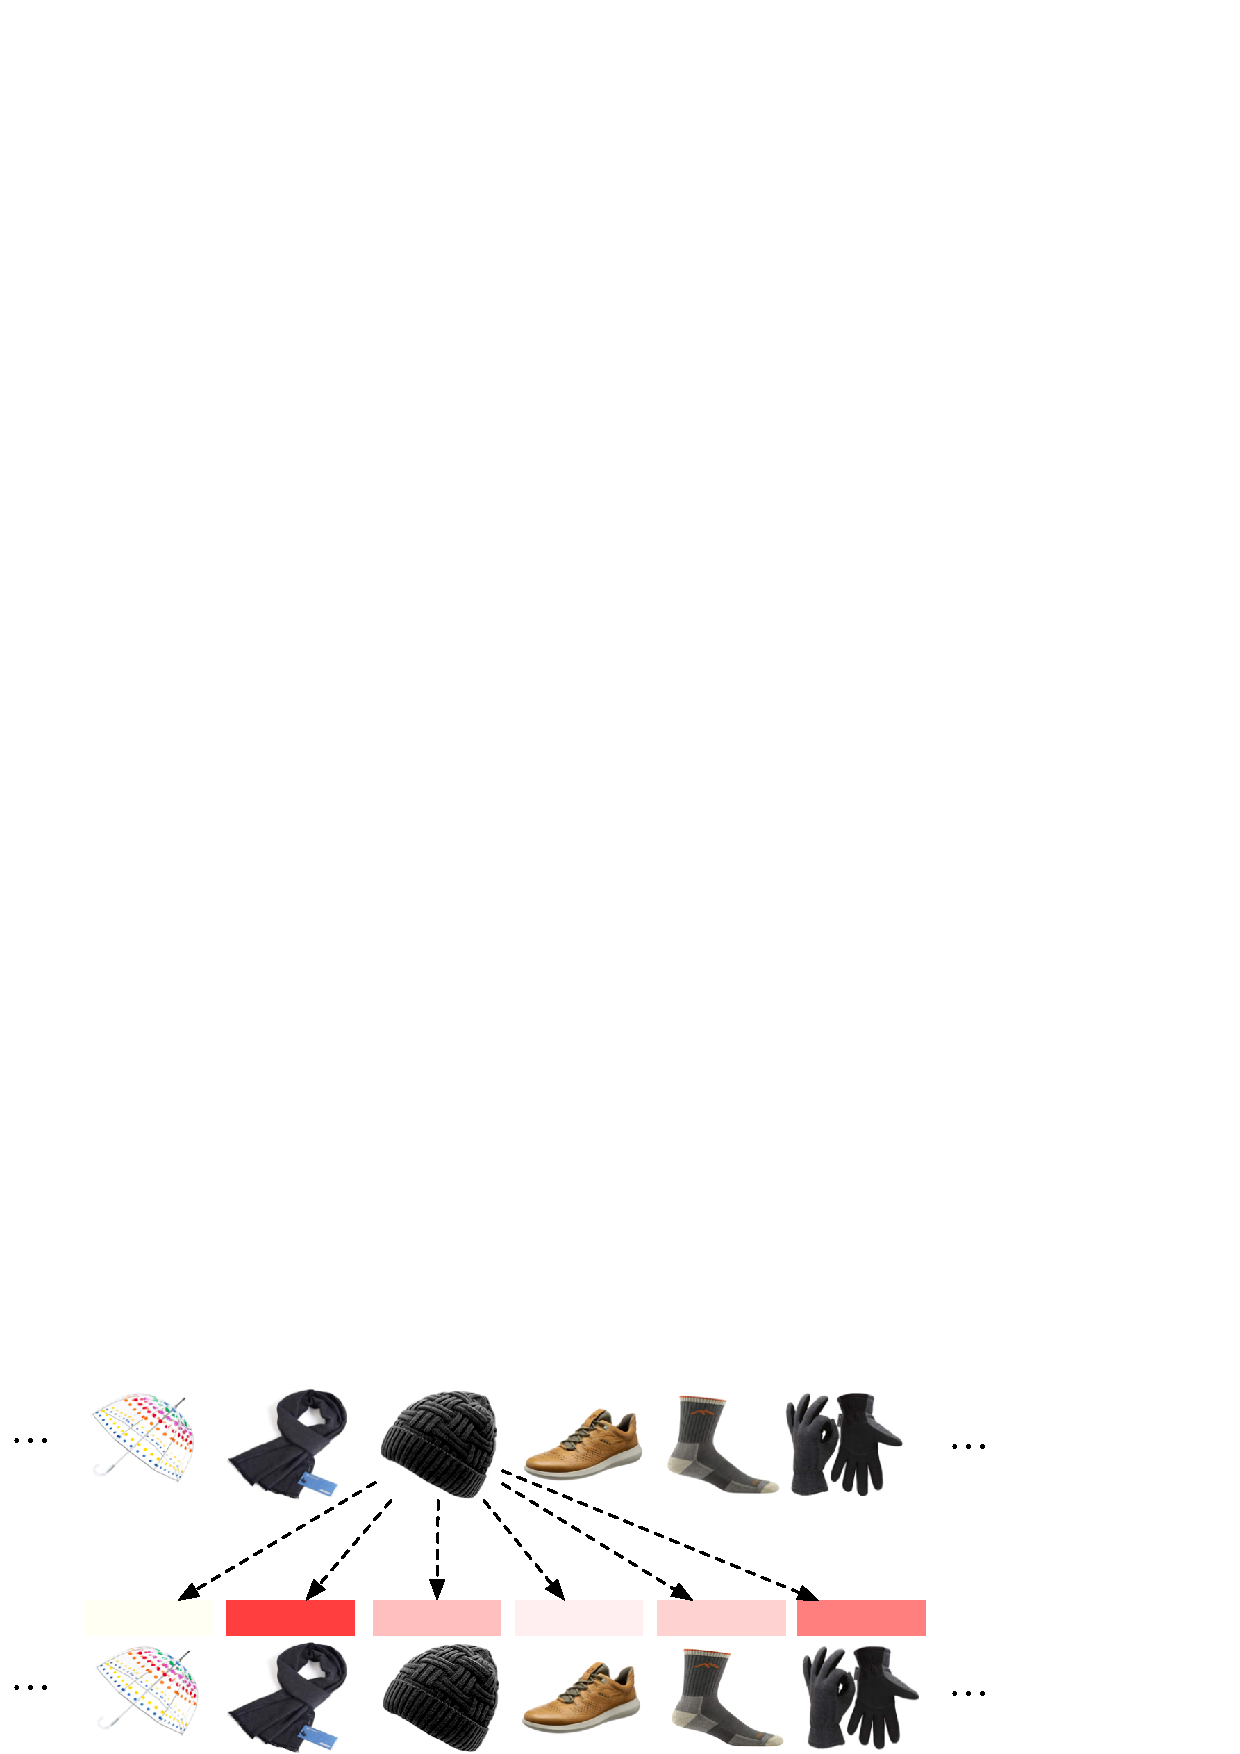
\includegraphics[width=1.0\columnwidth]{figure/attention.pdf}}
	\caption{Attention weight visualization. \textit{AtLocation} is required for prompt in the left column and \textit{PartOf} is required for prompt in the right column.} \label{fig:attention}
\end{figure}
Specifically, we focus on the attention weights between [MASK] token and 
other tokens in the prompt. A first glance of change of attention pattern 
is given in \figref{fig:LAMA} and we show more examples of other ConcetpNet 
relations in \figref{fig:attention}. We observe that while the original 
pretrained model tends to attend to special tokens like period and [SEP], 
the subnetwork successfully grasps the relevant concepts~(i.e., apple, 
worms, and basement) in the prompt hence produces the right object. 
We also use t-SNE~\citep{vanDerMaaten2008} to visualize the last layer's 
representation of [CLS] for each prompt. From \figref{fig:tsne}, the 
representations computed by original pretrained model are hardly separable as 
different types of knowledge are mixed together. In contrast, the pruned 
subnetwork can extract meaningful and disentangled representations for 
different commonsense relations.

\begin{figure}[th]
	\centering
	\scalebox{1.0}{\includegraphics[width=1.0\columnwidth]{figure/tsne_compare.pdf}}
	\caption{t-SNE visualization of [CLS]'s representation from original~(left) and pruned~(right) \textsc{BERT-base}.} \label{fig:tsne}
\end{figure}


\subsection{Commonsense Knowledge Base Completion~(CKBC)}
\label{sec:ckbc}
We evaluate the utility of identified relation-specific subnetworks on CKBC in an unsupervised manner. Specifically, we use the ConceptNet-100K benchmark provided by \citet{Li2016}. To ensure a fair evaluation, 
we manually create a subset of ConceptNet-100K 
consisting of triples with single-token subject/object. We also ensure that its dev/test set has \textbf{no overlap} with C-LAMA.
Each relation is associated with a sentence template~(provided in 
Appendix)~\citep{Kwon2019} of which the wording is distinct from 
those in C-LAMA. We acknowledge that these sentence templates might be suboptimal for certain relations, but prompt optimization is 
out of the scope of this paper. The resulting dataset contains 
$17,891$ training instances, $349$ development instances, 
and $446$ test instances.

\textbf{Link prediction.}~~We first formulate CKBC as a link prediction task 
and compare subnetworks~(i.e., $\mathcal{LM}_{\theta_r}$ 
is queried to predict missing link for instance of relation $r$) as well as original PLMs
against strong supervised KB completion mothods. 


\tabref{table:linkprediction} shows the results. Most of the supervised 
models outperform full-scale PLMs by a large margin, which suggests the 
inefficacy of directly using PLMs to perform link prediction. However, 
the subnetworks identified by our pruning procedure can
acquire performance on par with or better than state-of-the-art 
supervised models. Surprisingly, the pruned \textsc{DistilBERT} get the 
highest MRR, outperforming other larger and more advanced PLMs. 
\textsc{RoBERTa} struggles to predict correct objects, perhaps due to 
its larger vocabulary size compared to WordPiece~($50,265$ vs $30,522$) 
and less lexicon overlap~($53\%$ vs $59\%$) with the dataset.

%\KZ{It seems that our method (pruned models) don't work so well in the
%test set, compared to dev set. The scores for the same model between dev set and
%test set are also quite diff. Can you explain in this para?}

\textbf{Triple classification}~~We can also formulate CKBC as a triple classification task. Following ~\citet{Feldman2020}, we use estimated point-wise mutual information~(PMI) computed by pretrained language model as a surrogate of a triple's validity. An expectation-maximization-based Gaussian mixture clustering method is used and instances in the cluster with higher mean PMI are labeled as valid. 
\begin{table}[t]
	\centering
	\scriptsize
	\begin{tabular}{l|c}
		\toprule
		\textbf{Model} &  \textbf{F1 Score}\\
		\midrule
		\textsc{DistilBERT} & 74.1\\
		\textsc{DistilBERT}~(pruned) & \textbf{76.3}\\
		\midrule
		\textsc{BERT} & 73.7\\
		\textsc{BERT}~(pruned) & \textbf{76.7}\\
		\midrule
		\textsc{RoBERTa} &74.8 \\
		\textsc{RoBERTa}~(pruned) & \textbf{76.9}\\
		\midrule
		\textsc{MPNet} &76.5 \\
		\textsc{MPNet}~(pruned) & \textbf{78.0}\\
		\bottomrule
	\end{tabular}
	\caption{Triple classification on ConceptNet-100K.}
	\label{table:tripleclassification}
\end{table}
In our preliminary experiments, we found that the model pruned by the mask 
of a single relation might not be robust for PMI estimation and generally 
performed inferior to the intact model. 
In the same spirit as model ensembling, we then perform grid search over 
combinations of multiple knowledge, which is similar to what we did 
in zero-shot commonsense reasoning. For all four PLMs considered in 
\tabref{table:tripleclassification}, we observe that there exists one 
or multiple knowledge combinations delivering F1 score higher than the 
original models. 
%\KZ{Why is the difference between pruned and unpruned models
%not so big compared to link prediction?}

\textbf{Triple extraction.}~~We then investigate the ability of specialized 
subnetworks to extract novel commonsense knowledge triples absent 
from the dataset. We randomly sample 100 triples from the test set of 
ConceptNet-100K and for each sample use top-$K$ predictions from 
pruned \textsc{DistilBERT-base} as candidate objects. 
Three human annotators are asked to first determine the correctness of 
each candidate object and further determine their novelty~(i.e., not present 
in any of train/validation/test set) if deemed to be correct. 
The Fleiss Kappa inter-annotator agreement $\kappa$ is 0.66/0.65 
for precision and novelty, respectively.
\begin{figure}[t]
	\centering
	\scalebox{0.7}{\includegraphics[width=1.0\columnwidth]{figure/precision_novelty_2.pdf}}
	\caption{Precision-novelty curve with varied $K$.} \label{fig:extraction}
\end{figure}
\figref{fig:extraction} shows the change of precision-novelty with varied $K$. We observe a clear trade-off between the validity and novelty of triples extracted by the pruned model. As expected, a large $K$ inevitably makes noisy predictions but is more likely to extract unseen knowledge. For the purpose of knowledge enrichment, one might choose a large $K$ to ensure a desirable recall. We list the obtained novel triples in the Appendix D due to space limits.






\subsection{Commonsense Reasoning~(CSR)}
\label{sec:csr}
After identifying sparse subnetworks within PLMs that specialize in different commonsense knowledge, we now evaluate their generalization ability in the context of commonsense reasoning.
%One desirable outcome of our pruning procedure is the transformation from language representation to knowledge representation. We test if such subnetworks generalize in the context of commonsense reasoning.

\textbf{Many-shot learning.}~~We experiment with \textsc{BERT-base} and its deterministically pruned version using supervised fine-tuning on $7$ datasets: RTE~\citep{CambridgeJournals:6906264}, COPA~\citep{roemmele_choice_2011}, CommonsenseQA~\citep{talmor-etal-2019-commonsenseqa}, SWAG~\citep{zellers-etal-2018-swag}, HellaSWAG~\citep{DBLP:journals/corr/abs-1905-07830},   aNLI~\citep{DBLP:journals/corr/abs-1908-05739} and CosmosQA~\citep{huang-etal-2019-cosmos}. For each task, we identify the commonsense knowledge it might requires with a simple heuristic. Specifically, we obtain the five most frequent relations~(measured by how many times subject and object of certain relation appear in the context or answer) for each task and perform grid search over the combinations of these relationns. Then we take the union of masks for each relation and apply the resultant mask to the BERT as initialization for finetuning.
We repeat the training three times with different random seeds for each task. 
The  choice of mask combination for each task can be found in Appendix B.

The results in \tabref{table:finetuning} shows that, when initialized with proper weights, the model can be better fine-tuned on downstream commonsense reasoning tasks via more useful \textit{prior} knowledge. We further analyze the change of performance under the low-resource regime on COPA dataset. \figref{fig:copa} shows that the pruned \textsc{BERT} exhibits a notable advantage when training data is extremely scarce. As more training data is seen, the benefit of the pruned 
model becomes less prominent, i.e., $p>0.05$.
\begin{table}[t!]
	\centering
	\scriptsize
	\begin{tabular}{l|cc|c}
		\toprule
		\textbf{Task} & \textbf{Original} & \textbf{Pruned} &$p$-value \\
		\midrule
		RTE & 69.2$\pm${\scriptsize 2.3} & 69.8$\pm${\scriptsize2.0}& 0.12\\

		COPA & 62.4$\pm${\scriptsize 5.0} & 63.0$\pm${\scriptsize 4.7} &0.33  \\

		CommonsenseQA & 53.1$\pm${\scriptsize 0.6} & 54.1$\pm${\scriptsize 0.7} &0.08\\

		SWAG & 73.9$\pm${\scriptsize 0.3} & 74.2$\pm${\scriptsize 0.1} &0.09\\
		HellaSWAG & 38.9$\pm${\scriptsize 0.4} & 39.1$\pm${\scriptsize 0.5}&0.32  \\
		aNLI &63.7$\pm${\scriptsize 0.4} &64.0$\pm${\scriptsize 0.4}  &0.19\\
		CosmosQA &61.3$\pm${\scriptsize 1.0} &61.8$\pm${\scriptsize 0.2} &0.26\\
		\bottomrule
	\end{tabular}
	\caption{Finetuning results of \textsc{BERT} for CSR.}
	\label{table:finetuning}
\end{table}
\begin{figure}[t]
	\centering
	\scalebox{0.75}{\includegraphics[width=1.0\columnwidth]{figure/copa.pdf}}
	\caption{Finetuning result of \textsc{BERT} on COPA with varying portion of data.} \label{fig:copa}
\end{figure}
\begin{table*}[t!]
	\centering
	\scriptsize
	\begin{tabular}{l|cccccccc|c}
		\toprule
		\textbf{Model} &COPA-Tra. &COPA-Val. &CSQA &CA &WSC  &SM &ARCT1 &ARCT2 &Avg. \\
		\midrule
		\textsc{DistilBERT} &58.3 &60.0 &29.6 &84.6 &53.3  &71.6 &48.6 &50.4  &57.0  \\
		\textsc{DistilBERT}~(pruned) &\textbf{61.5} &\textbf{69.0} &\textbf{31.5} &\textbf{89.6} &\textbf{56.9}  &\textbf{72.1} &\textbf{53.4} &\textbf{51.6} & \textbf{60.7} \\
		\midrule
		\textsc{BERT} &60.2 &54.0 &26.5 &89.0 &57.3  &69.7 &46.8 &50.3 &56.7 \\
		\textsc{BERT}~(pruned) &\textbf{63.0} &\textbf{64.0} &\textbf{28.5} &\textbf{91.8} &\textbf{59.0}  &\textbf{71.7} &\textbf{50.0} &\textbf{52.0}  & \textbf{60.0}\\
		\midrule
		\textsc{RoBERTa} &60.7 &59.0 &39.9 &90.1 &61.8  &73.1 &48.6 &53.1 &60.7 \\
		\textsc{RoBERTa}~(pruned) &\textbf{65.3} &\textbf{72.0} &\textbf{40.4} &\textbf{93.4} &\textbf{62.9}  &\textbf{74.4} &\textbf{53.2} &\textbf{55.1} &\textbf{64.6}\\
		\midrule
		\textsc{MPNet} &66.5 &69.0 &40.0 &94.5 &64.3&75.8  &52.9 &56.7 &64.9  \\
		\textsc{MPNet}~(pruned) &\textbf{71.0} &\textbf{74.0} &\textbf{41.7} &\textbf{97.3} &\textbf{66.4}  &\textbf{77.5} &\textbf{56.1} &\textbf{57.7}  & \textbf{67.7}\\
		\bottomrule
	\end{tabular}
	\caption{Zero-shot results of accuracy~(\%) on commonsense reasoning tasks. Better results of each pair is in \textbf{bold}.}
	\label{table:zeroshot}
\end{table*}



\textbf{Zero-shot learning.}~~We next assess the ability of specialized 
subnetworks to perform zero-shot commonsense reasoning, a setting where 
the knowledge relied on to complete the task is solely determined by the model 
parameters. Here we focus on the following multiple-choice datasets: training set of COPA~(COPA-Tra.), validation set of COPA~(COPA-Val.), CommonsneseQA, Conjunction 
Acceptability~(CA)~\citep{Zhou2019}, 
Winograd Schema Challenge~(WSC)~\citep{levesque_winograd_2012}, 
SenseMaking~(SM)~\citep{wang-etal-2019-make}, 
ARCT1~\citep{habernal-etal-2018-argument} and 
ARCT2~\citep{DBLP:journals/corr/abs-1907-07355}. Each sample in the above datasets can be formulated as $\{[CLS]~context~[SEP]~choice_i ~[SEP]\}_{i=1}^{N}$, where $i$ is the subscript and $N$ is the number of choices. We compute the plausibility score of each choice using MLM head. Choice with the highest plausibility score is chosen as the answer. 

Since multiple types of knowledge are typically required for effectively 
reasoning over concepts, for each task, we perform grid search over 
combinations of $3$-$4$ different commonsense knowledge out of 
the $16$ total types and reported the best accuracy in \tabref{table:zeroshot}. 
We put the best combination for each model on each task in Appendix B
for space constraints. By combining multiple commonsense knowledge useful for the task, 
we show that the pruned models can actually surpass their full-scale 
version in all tasks considered in our experiments. 
The most likely explanation is that knowledge irrelevant to the specific task 
in the original models hurt the in-domain zero-shot reasoning capability. 
It also manifests that the most important reasoning skills vary from 
task to task.

\section{Related Work}
\paragraph{Language models for phonetic reconstruction}
A related task of phonological ancient language reconstruction is proto-word reconstruction, which takes set of words in different contemporary languages as input and the corresponding word in their common ancestral language as result of supervised reconstruction. ~\citet{meloni_ab_2021} and~\citet{akavarapu_cognate_2023} both evaluate neural networks' performance on Romance language family's reconstruction task. ~\citet{kim_transformed_2023} first introduce Transformer architecture into proto-word reconstruction task and outperforms previous models on both Romance and Sinitic dataset. 
While large language models (LLMs) have recently demonstrated exceptional capabilities in understanding and generating contemporary languages, their proficiency in comprehending ancient Chinese, remains inadequate. \citet{zhang-li-2023-large}'s research highlights the limitations of LLMs in handling the complex ancient Chinese phonetic information.
\paragraph{Chinese phonetic dataset}
In terms of Chinese phonetic datasets, current digitization all organize the ancestor language (Middle Tang Chinese) and its daughter languages (modern Chinese dialects) into a cognate set. ~\citet{hou_j_xiandai_2004} first collecte 2,789 cognates of word-wise Chinese dialect pronunciation. ~\citet{chang_wikihan_2022} expand Hou's dataset, organize entries by characters instead of word.
As for chronological phonology dataset in Chinese, existing resources are mainly from studies of historical linguistics. Swedish sinologist Karlgren first put forward the phonological reconstruction of Middle Tang Chinese~\cite{TheReconstructionofAncientChinese}. ~\citet{wang_l_hanyu_2012} provides a comprehensive analysis of Chinese language phonological evolution. However, these sources are not digitized to our knowledge.
\section{Conclusion}
We implement a novel sequence-based dependency parsing
framework which takes advantage of high order features 
in parsing history. 
%We can also adapt beam search to this framework so as to
%relax the strictly greedy nature. Vine pruning\cite{rush2012vine} could
%be incorporated to speed up the parsing.
More importantly, we discovered that the parsing accuracy is very sensitive to
the quality of parsing sequence. Future work can be focused on
developing better sequence predictors that outperform Malt action classifier.
Furthermore, we use two sets of features for sequence predictor and
head mapper right now. A unified set of features between these two components
are worth exploring.
%Besides, better sequence predicting method and unified feature
%representation of two components are worth exploring.
%
%Though we currently get a not bad result,
%the sequence predictor still needs more exploration.
%According to our experiment, slightly changes
%on the sequence can lead to a fatal decline on accuracy. Ensuring the match degree of training sequence and testing
%sequence demands a high quality of sequence predictor.
%
%Further, the features in our current implementation are not expanded and well tuned yet  and we are free to define high order features to make use of parsing history. Our framework is flexible to merge other technics to enhance the performance. Introducing beam could make up for our greedy decoder and improve our accuracy. Vine pruning\cite{rush2012vine} could speed up parsing process. Besides, better sequence predicting method and unified feature representation of two components are worth exploring.

\section{Ethical Statement}
In this work, we make every effort to minimize the risk of personal privacy leakage during the data collection process. We replaced usernames with random identifiers to prevent identification of users without external information. All datasets used in our study are either publicly available or adhere to their respective licenses. We sign and comply with the data use agreement to prevent privacy infringement or other potential misuses. All posts in examples were de-identified and paraphrased for anonymity.
What's more, we carefully considered the application of social media for the detection of mental illnesses. The purpose of this work is not to replace psychiatrists. Instead, we hope our model will be used as an effective auxiliary tool by experienced psychiatrists in the future.
% \begin{figure}[t]
% \centering
% 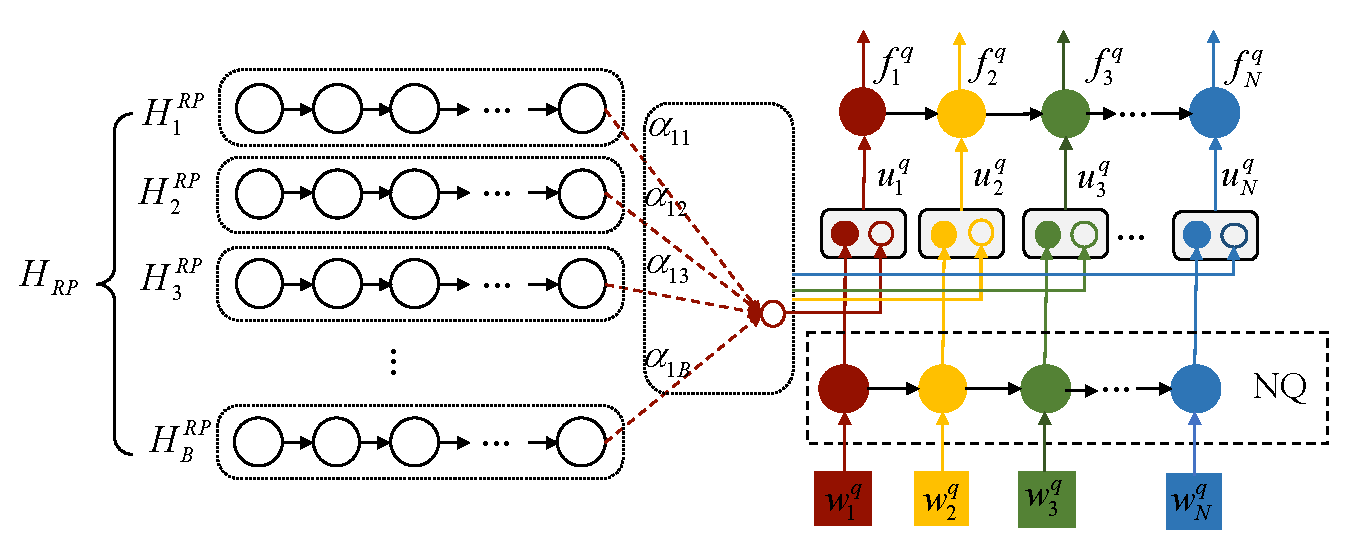
\includegraphics[width=0.9\columnwidth]{figure1} % Reduce the figure size so that it is slightly narrower than the column. Don't use precise values for figure width.This setup will avoid overfull boxes.
% \caption{Using the trim and clip commands produces fragile layers that can result in disasters (like this one from an actual paper) when the color space is corrected or the PDF combined with others for the final proceedings. Crop your figures properly in a graphics program -- not in LaTeX.}
% \label{fig1}
% \end{figure}

% \begin{figure*}[t]
% \centering
% 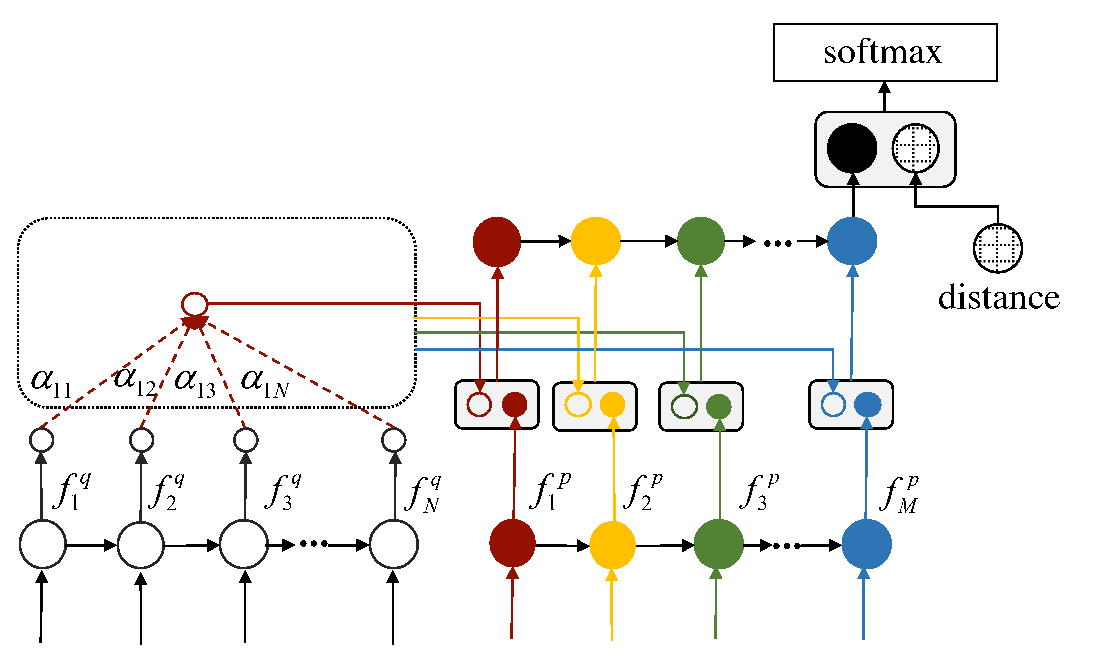
\includegraphics[width=0.8\textwidth]{figure2} % Reduce the figure size so that it is slightly narrower than the column.
% \caption{Adjusting the bounding box instead of actually removing the unwanted data resulted multiple layers in this paper. It also needlessly increased the PDF size. In this case, the size of the unwanted layer doubled the paper's size, and produced the following surprising results in final production. Crop your figures properly in a graphics program. Don't just alter the bounding box.}
% \label{fig2}
% \end{figure*}

% Using the \centering command instead of \begin{center} ... \end{center} will save space
% Positioning your figure at the top of the page will save space and make the paper more readable
% Using 0.95\columnwidth in conjunction with the



% \appendix
% \section{Reference Examples}
% \label{sec:reference_examples}

% \nobibliography*

% \paragraph{Website or online resource~\nocite{c:23}} Use the \texttt{@misc} class. Add the url in the \texttt{howpublished} field and the date of access in the \texttt{note} field:
% \begin{quote}
% \begin{footnotesize}
% \begin{verbatim}
% @misc(key,
%   [...]
%   howpublished="\url{http://...}",
%   note="Accessed: YYYY-mm-dd",
% )
% \end{verbatim}
% \end{footnotesize}
% \end{quote}
% \bibentry{c:23}.

\bibliography{aaai25}

\input{checklist.tex}

\end{document}
